\chapter[Resultados e Discussão]{Resultados e Discussão}

\section{Descrição}

A cada iteração "\textit{i}", um subconjunto candidato de \textit{i} variáveis é determinado. O melhor subconjunto é aquele que minimiza o erro LOOCV. É importante reiterar que o algoritmo utiliza uma estratégia de \textit{greedy search} para buscar os subconjuntos e, portanto, a otimalidade global desses subconjuntos não é garantida.

O algoritmo foi aplicado a cada um dos bancos de dados indicados na sessão anterior, de maneira a determinar subconjuntos otimizados de variáveis para uso em um modelo de regressão. Os gráficos obtidos demonstram, a cada iteração, a variável ainda não utilizada que, ao ser acrescentada no modelo, traz a maior redução do erro de validação cruzada (ou o menor aumento). 

Para verificar o efeito da utilização do grupo de entradas proposto, duas redes neurais foram treinadas em cada conjunto de dados. Uma utilizando a totalidade das variáveis disponíveis e outra o subconjunto sugerido pelo algoritmo. Os parâmetros de treinamento, tais como taxa de aprendizado e tamanho da camada oculta, foram determinados e fixados por conjunto de dados, permitindo a comparação do efeito isolado da variação do conjunto de entradas.



\section{Seleção de Variáveis}

\subsection{\textit{Communities and Crime}}

No banco de dados \textit{Communities and Crime}, o erro de validação cruzada LOOCV mínimo foi observado em um conjunto com apenas 37 das 102 variáveis. A adição de variáveis posteriormente teve pouca influência no erro de validação cruzada, com uma tendência à degradação da performance na inclusão das últimas variáveis.

O resultado para cada iteração pode ser verificado na figura \ref{fig:stepwise_CommunitiesandCrime_validation}.

\begin{figure}[!htb]
    \centering
    \caption{Seleção de Variáveis \textit{Stepwise: Communities and Crime}.}
    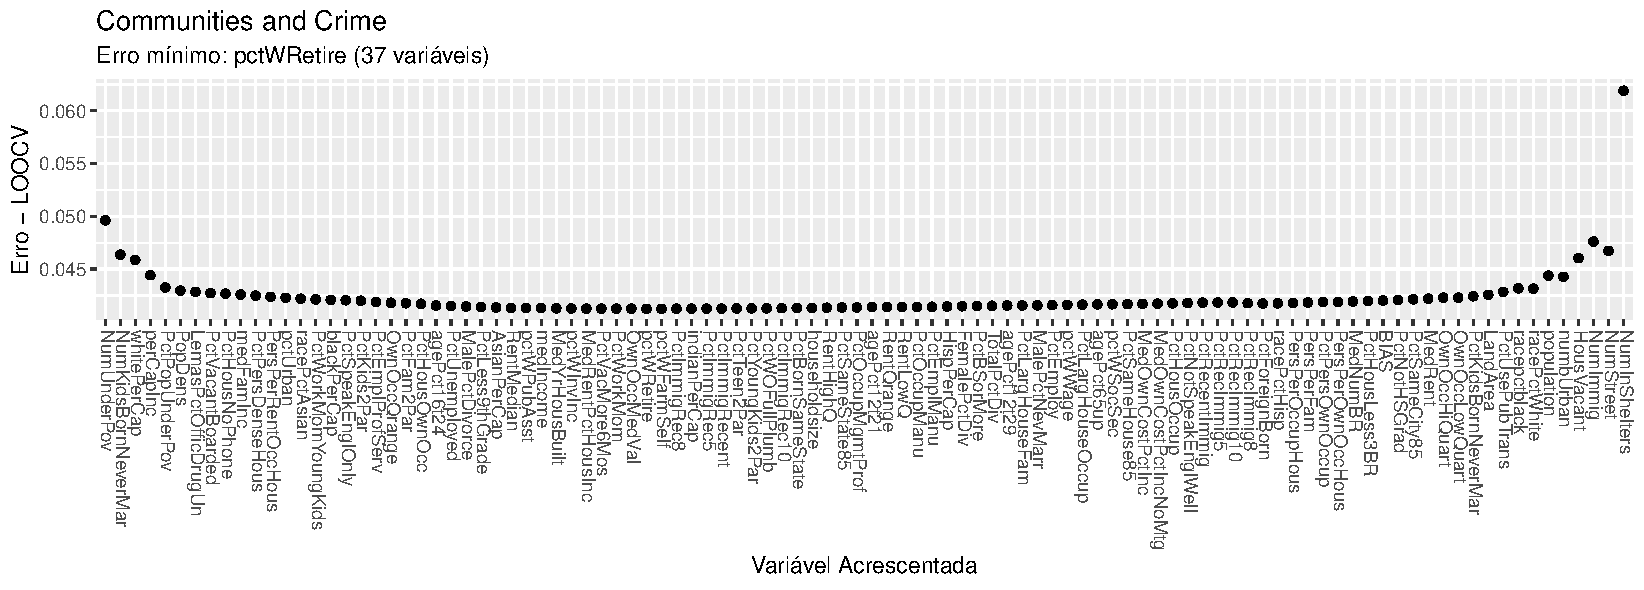
\includegraphics[height=163pt]{imgs/res/CommunitiesandCrime_validation.pdf}
    \legend{Fonte: Própria.}
    \label{fig:stepwise_CommunitiesandCrime_validation}
\end{figure}
\FloatBarrier

\subsection{\textit{Forest Fires}}
No banco de dados \textit{Forest Fires}, o erro de validação cruzada LOOCV mínimo foi observado em um conjunto com apenas 4 das 12 variáveis. A adição de variáveis posteriormente resultou em perda significativa de performance. 

O resultado para cada iteração pode ser verificado na figura \ref{fig:stepwise_ForestFiresDataset_validation}.

\begin{figure}[!htb]
    \centering
    \caption{Seleção de Variáveis \textit{Stepwise: Forest Fires}.}
    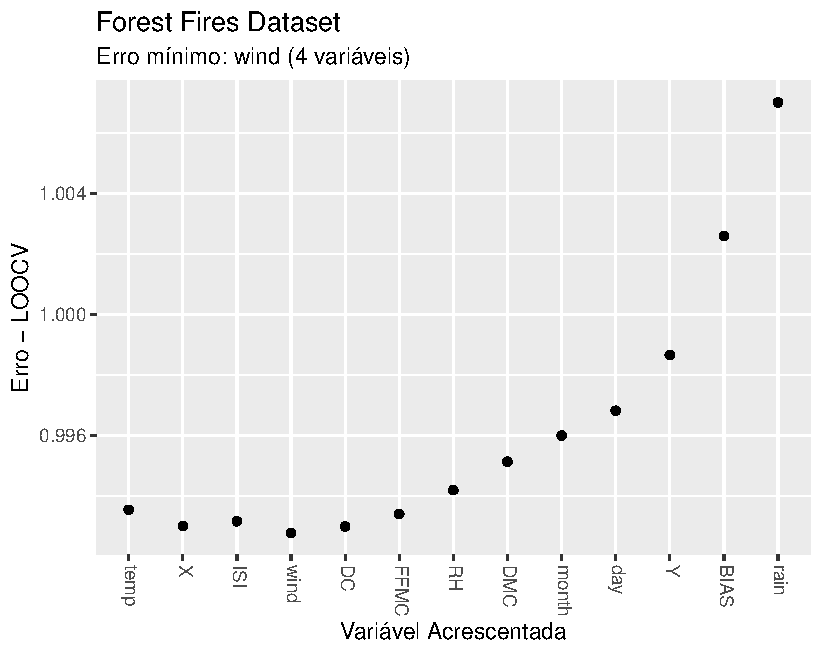
\includegraphics[height=200pt]{imgs/res/ForestFiresDataset_validation.pdf}
    \legend{Fonte: Própria.}
    \label{fig:stepwise_ForestFiresDataset_validation}
\end{figure}
\FloatBarrier

\subsection{\textit{USA Housing}}
No banco de dados \textit{USA Housing}, o erro de validação cruzada LOOCV mínimo foi observado em um conjunto com apenas 35 das 80 variáveis. A adição posterior de variáveis teve pouca influência no erro de validação cruzada. 

O resultado para cada iteração pode ser verificado na figura \ref{fig:stepwise_USAHousingDataset_validation}.

\begin{figure}[!htb]
    \centering
    \caption{Seleção de Variáveis \textit{Stepwise: USA Housing}.}
    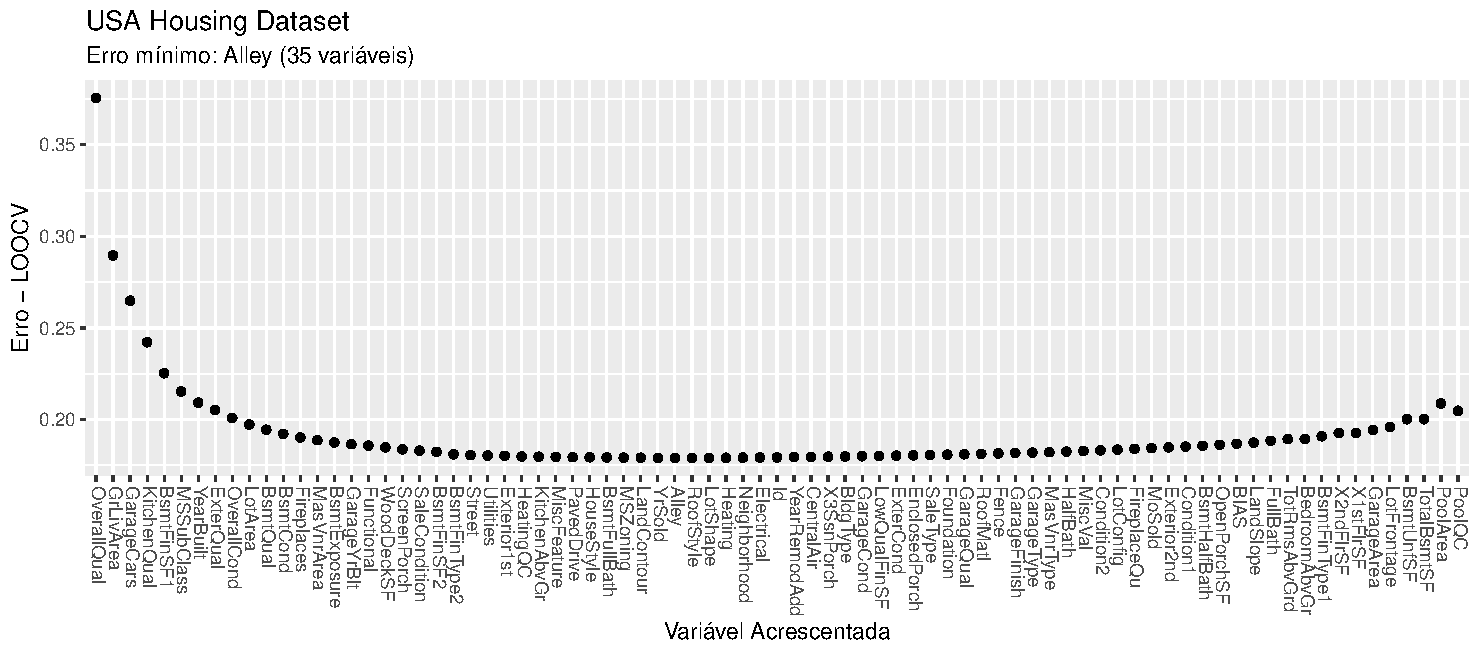
\includegraphics[height=200pt]{imgs/res/USAHousingDataset_validation.pdf}
    \legend{Fonte: Própria.}
    \label{fig:stepwise_USAHousingDataset_validation}
\end{figure}
\FloatBarrier

\subsection{\textit{Wisconsin Breast Cancer}}
No banco de dados \textit{Wisconsin Breast Cancer}, o erro de validação cruzada LOOCV mínimo foi observado em um conjunto com apenas 8 das 32 variáveis, e foi identificada também uma perda significativa de performance quando utilizado um subconjunto candidato de mais de 16 variáveis. 

O resultado para cada iteração pode ser verificado na figura \ref{fig:stepwise_WisconsinBreastCancer}.

\begin{figure}[!htb]
    \centering
    \caption{Seleção de Variáveis \textit{Stepwise: Wisconsin Breast Cancer Dataset}.}
    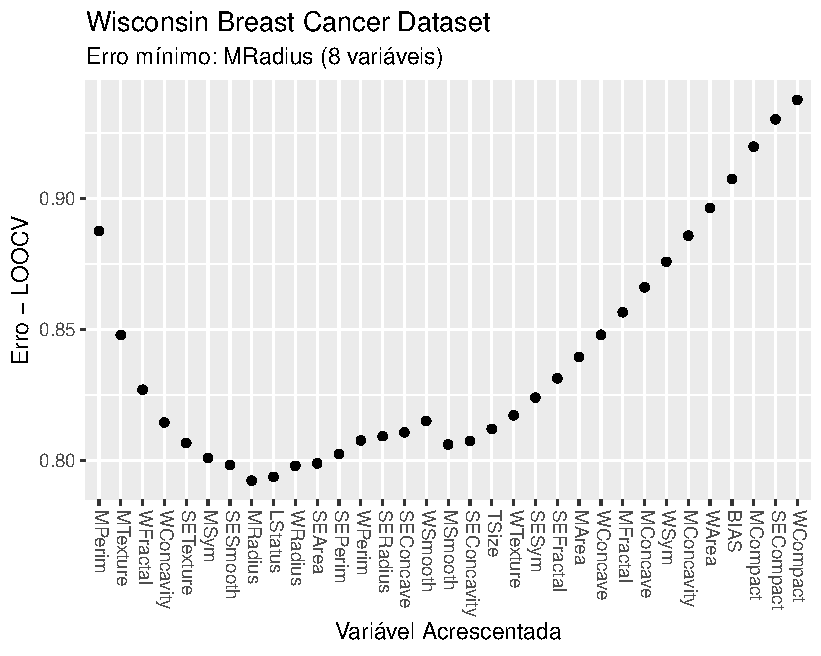
\includegraphics[height=200pt]{imgs/res/WisconsinBreastCancerDataset_validation}
    \legend{Fonte: Própria.}
    \label{fig:stepwise_WisconsinBreastCancer}
\end{figure}
\FloatBarrier

\subsection{Discussão}
Observou-se o decréscimo do erro com o aumento do número de variáveis selecionadas até um ponto de mínimo, a partir do qual a tendência se inverte e o erro passa a aumentar. Tal dinâmica é esperada, uma vez que o aumento do número de parâmetros, na regressão linear, resulta no aumento da complexidade do modelo \cite[p. 224]{statistical_learning}, o que por sua vez pode reduzir a capacidade de generalização do modelo. 

De fato, ao se reduzir a complexidade do modelo através do aumento do parâmetro de regularização ($\lambda$), observa-se a diminuição da tendência ao overfitting, conforme demonstra a figura \ref{fig:lambda_WisconsinBreastCancer}.

\begin{figure}[!htb]
    \centering
    \caption{Efeito do parâmetro de regularização ($\lambda$): \textit{Wisconsin Breast Cancer Dataset}.}
    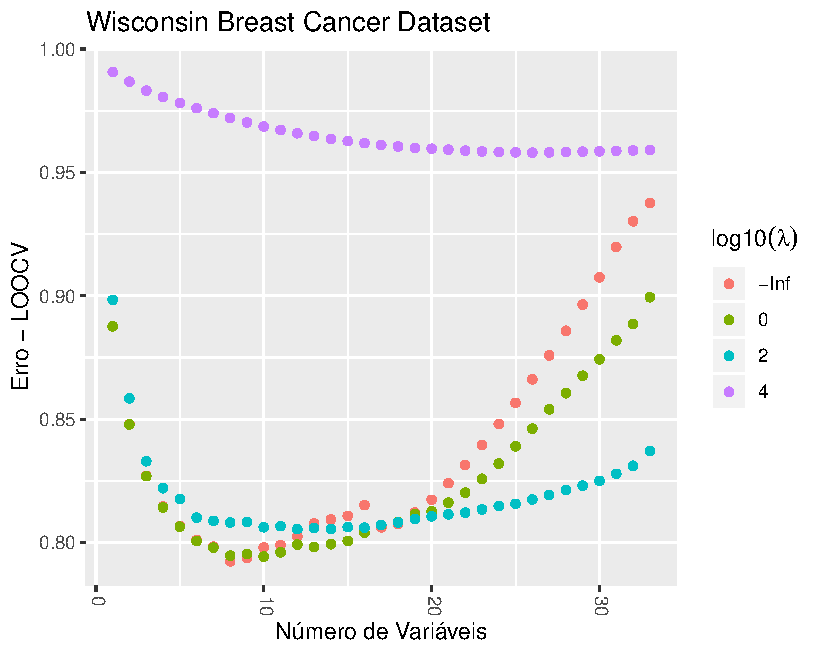
\includegraphics[height=200pt]{imgs/res/WisconsinBreastCancerDataset_lambda}
    \legend{Fonte: Própria.}
    \label{fig:lambda_WisconsinBreastCancer}
\end{figure}

É interessante notar que valores baixos de $\lambda$ tiveram pouca ou nenhuma influência nos primeiros subconjuntos ótimos selecionados pelo algoritmo, alterando apenas a seleção na região com tendência ao overfitting. Dessarte, a utilização de um parâmetro de regularização não nulo de pequena magnitude tem pouca influência no conjunto selecionado, enquanto melhora a estabilidade numérica do método, evitando operações com matrizes singulares.


\FloatBarrier
\section{Modelos}

\subsection{\textit{Communities and Crime}}

\begin{table}[!htb]
    \caption{Parâmetros de Treinamento: \textit{Communities and Crime}.}
    \begin{center}        
        \begin{tabular}{@{}ll@{}}
        \toprule
                            & Conjunto de dados \\ \midrule
        Tamanho (neurônios)     & 10                \\
        Taxa de Aprendizado   & 1e-4              \\
        Iterações             & 50                \\
        Função de Ativação    & ReLU              \\
        Conjunto de Validação & $30\%$            \\ \bottomrule
        \end{tabular}
    \end{center}
    \label{tbl:treinamento_comm_crime}
\end{table}

\begin{figure}[!htb]
    \centering
    \caption{Treinamento do Modelo: \textit{Communities and Crime}.}
    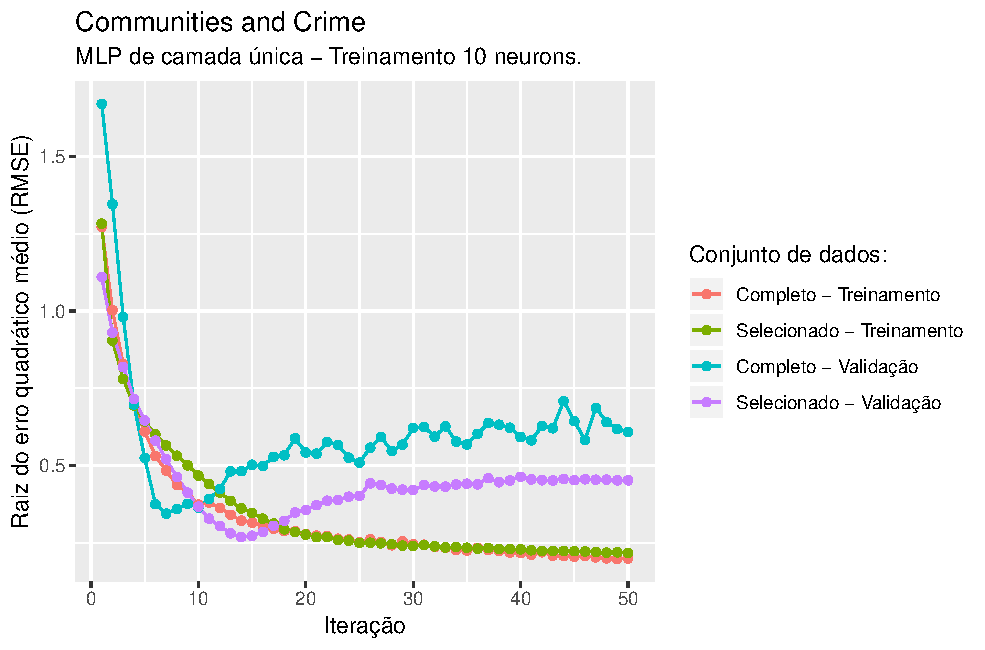
\includegraphics[height=200pt]{imgs/res/CommunitiesandCrime_model.pdf}
    \legend{Fonte: Própria.}
    \label{fig:modelo_CommunitiesandCrime_model}
\end{figure}

Observou-se que ambos os modelos apresentaram o mesmo erro de treinamento, porém, a rede neural treinada com o conjunto menor de variáveis de entrada apresentou melhor desempenho no conjunto de validação, indicando uma possível maior capacidade de generalização.


\FloatBarrier
\subsection{\textit{Forest Fires}}

\begin{table}[!htb]
    \caption{Parâmetros de Treinamento: \textit{Forest Fires}.}
    \begin{center}
        \begin{tabular}{@{}ll@{}}
        \toprule
                            & Conjunto de dados \\ \midrule
        Tamanho (neurônios)     & 5                 \\
        Taxa de Aprendizado   & 1e-4              \\
        Iterações             & 50                \\
        Função de Ativação    & Tanh              \\
        Conjunto de Validação & $30\%$            \\ \bottomrule
        \end{tabular}
    \end{center}
    \label{tbl:treinamento_forest}
\end{table}

\begin{figure}[!htb]
    \centering
    \caption{Treinamento do Modelo: \textit{Forest Fires}.}
    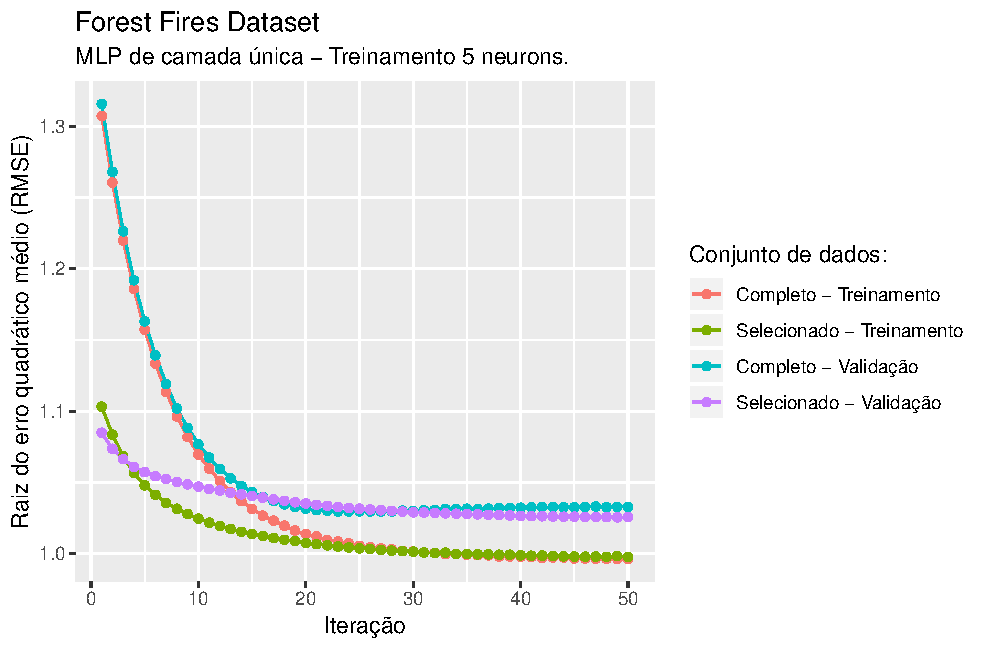
\includegraphics[height=200pt]{imgs/res/ForestFiresDataset_model.pdf}
    \legend{Fonte: Própria.}
    \label{fig:modelo_ForestFiresDataset_model}
\end{figure}


Os modelos treinados apresentaram desempenho similar, sendo que a versão que utiliza o conjunto restrito de entradas, apresentou uma convergência inicial mais rápida.

\FloatBarrier
\subsection{\textit{USA Housing}}

\begin{table}[!htb]
    \caption{Parâmetros de Treinamento: \textit{USA Housing}.}
    \begin{center}
        \begin{tabular}{@{}ll@{}}
        \toprule
                            & Conjunto de dados \\ \midrule
        Tamanho (neurônios)     & 10                \\
        Taxa de Aprendizado   & 1e-4              \\
        Iterações             & 50                \\
        Função de Ativação    & ReLU              \\
        Conjunto de Validação & $30\%$            \\ \bottomrule
        \end{tabular}
    \end{center}
    \label{tbl:treinamento_housing}
\end{table}

\begin{figure}[!htb]
    \centering
    \caption{Treinamento do Modelo: \textit{USA Housing}.}
    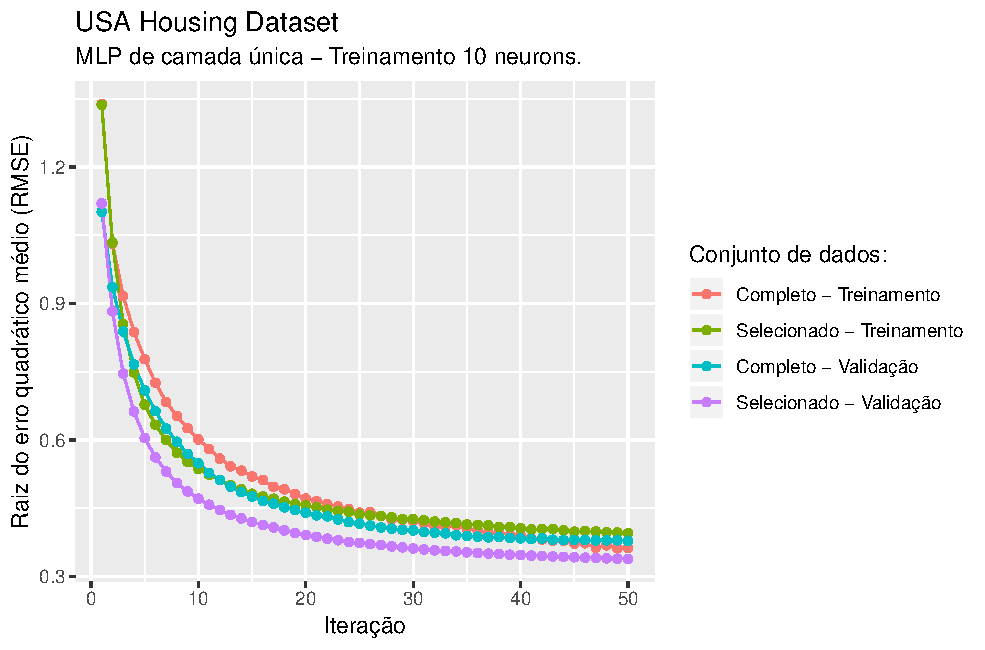
\includegraphics[height=200pt]{imgs/res/USAHousingDataset_model.pdf}
    \legend{Fonte: Própria.}
    \label{fig:modelo_USAHousingDataset_model}
\end{figure}

No conjunto de dados \textit{USA Housing}, as redes neurais apresentaram performance similar tanto para o caso de validação, quanto treinamento.

\FloatBarrier
\subsection{\textit{Wisconsin Breast Cancer}}

\begin{table}[!htb]
    \caption{Parâmetros de Treinamento: \textit{Wisconsin Breast Cancer}.}
    \begin{center}
        \begin{tabular}{@{}ll@{}}
        \toprule
                            & Conjunto de dados \\ \midrule
        Tamanho (neurônios)     & 10                \\
        Taxa de Aprendizado   & 1e-4              \\
        Iterações             & 50                \\
        Função de Ativação    & Tanh              \\
        Conjunto de Validação & $30\%$            \\ \bottomrule
        \end{tabular}
    \end{center}
    \label{tbl:treinamento_cancer}
\end{table}

\begin{figure}[!htb]
    \centering
    \caption{Treinamento do Modelo: \textit{Wisconsin Breast Cancer}.}
    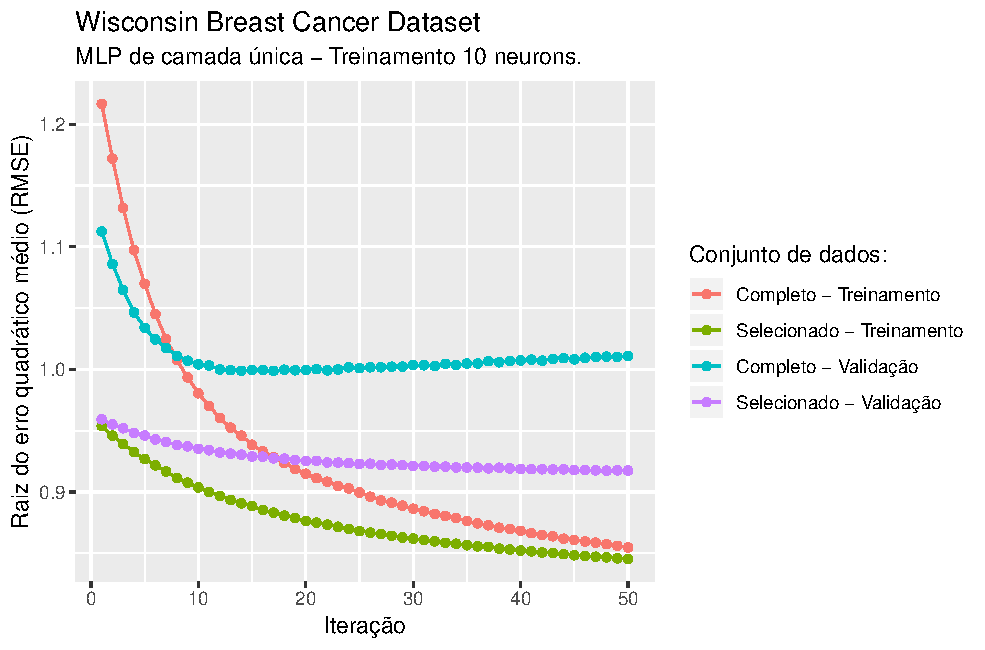
\includegraphics[height=200pt]{imgs/res/WisconsinBreastCancerDataset_model.pdf}
    \legend{Fonte: Própria.}
    \label{fig:modelo_WisconsinBreastCancerDataset_model}
\end{figure}

Por fim, no conjunto de dados \textit{Wisconsin Breast Cancer}, observou-se uma diferença expressiva entre o erro de validação e treinamento para o modelo que utiliza todas as entradas, indicando a ocorrência de \textit{overfitting}. Tal diferença foi reduzida, ao se utilizar o conjunto de variáveis selecionadas pelo algoritmo.

\FloatBarrier
\subsection{Discussão}

Em todos os dados avaliados, a utilização do conjunto de variáveis sugerido pelo algoritmo resultou em um modelo com performance similar ou superior ao que utiliza o conjunto completo.

Nota-se através da figura \ref{fig:modelo_CommunitiesandCrime_model} que, embora ambos modelos tenham demonstrado um padrão que sugere a presença de overfitting, o modelo com menos variáveis de entrada levou mais iterações para começar a exibir esse padrão e o apresentou em menor intensidade, uma vez que a para o mesmo erro de treinamento, seu erro de validação foi menor que sua contraparte com o conjunto completo de entradas. Na figura \ref{fig:modelo_ForestFiresDataset_model}, também é possível perceber essa tendência se iniciando nas últimas iterações do treinamento.

Na figura \ref{fig:modelo_USAHousingDataset_model}, não houve variações significativas ao se utilizar o modelo com número de entradas reduzido. Porém, na figura \ref{fig:modelo_WisconsinBreastCancerDataset_model}, observa-se que, embora os modelos tenham apresentado desempenho similar no erro de treinamento, houve uma melhora significava no erro de validação, sugerindo que a utilização do subconjunto proposto pelo algoritmo traz melhorias na capacidade de generalização do modelo para esse conjunto de dados.

Por fim é interessante ressaltar que os impactos da utilização de menos variáveis de entrada não se limitam a performance final do modelo. A redução da dimensão de entrada de um sistema tende a produzir modelos menores (com menos parâmetros), e consequentemente mais rápidos e simples de serem treinados.